\chapter{Workflow}
\section{Authentication}
The authentication uses JSON web tokens (JWT), which is a token-based authentication.\\
\begin{figure}[H]
    \centering
    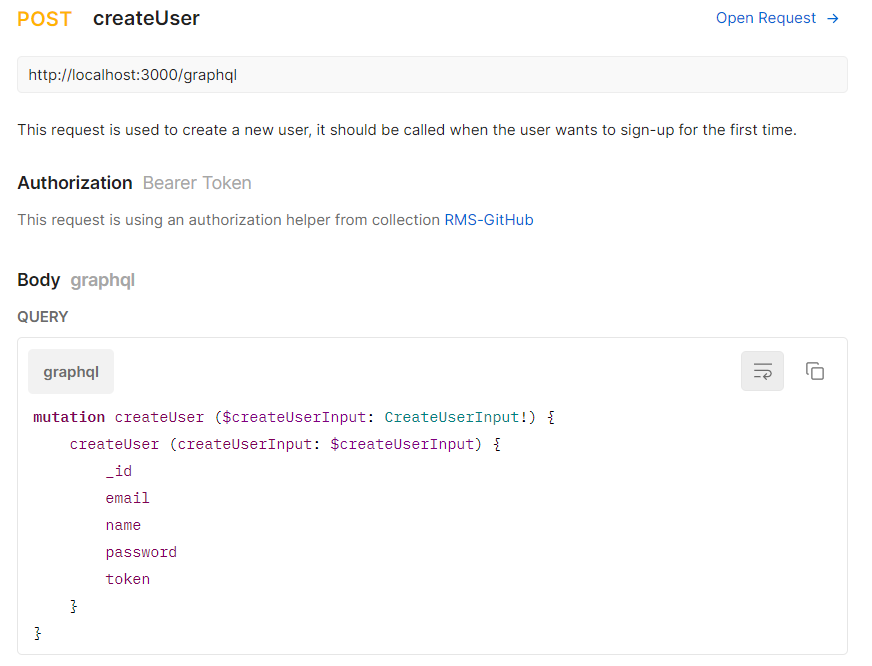
\includegraphics[scale=0.4]{images/createUserMutation.png}
    \caption{Sign-Up Mutation}
    \label{fig:tech-stack}
\end{figure}
If the user is a first time user, then this user must sign-up with their name, email-id and a password. After the user is successfully registered, he/she is give a token.\\
\begin{figure}[H]
    \centering
    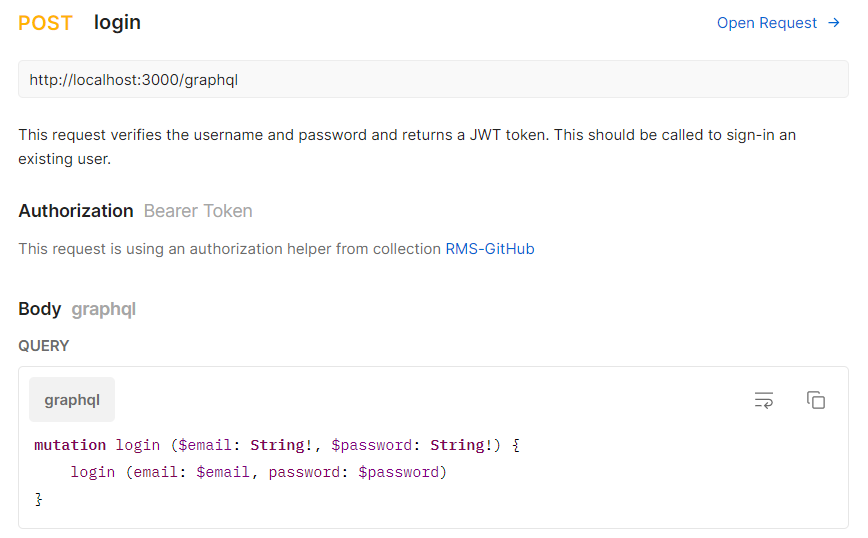
\includegraphics[scale=0.4]{images/loginMutation.png}
    \caption{Sign-In Mutation}
    \label{fig:tech-stack}
\end{figure}
If the user is an already existing user, then they must sign-in using their email-id and password, after a successful login, the server returns a token.\\
The token returned is stored in the local storage and for every request made by that user the token is attached to the header and validated in the server.\\
\begin{figure}[H]
    \centering
    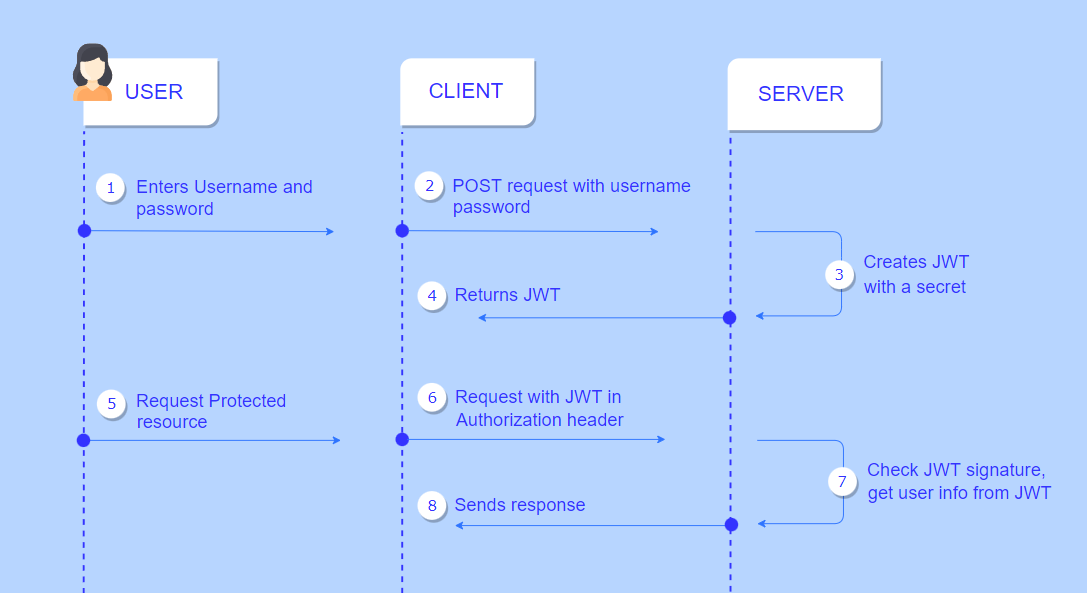
\includegraphics[scale=0.5]{images/auth-flow.png}
    \caption{Authentication Flow [\hyperref[lbl]{1}]}
    \label{fig:auth-flow}
\end{figure}

\section{Display}
The resource management system has three primary entities to show: the facilities, categories, and the items.

\subsection{Facility and Category}
The facilities and categories are shown as a grid view, with the facilities and categories shown as 
\subsection{Item}

\section{CRUD Operations}
\subsection{Facility and Category}
\subsection{Item}


